\documentclass[11pt]{jsarticle}
\usepackage{amsmath}
\usepackage{color}
\usepackage[dvipdfmx]{graphicx}
% https://qiita.com/BitPositive/items/6b13e2038d628c33be8e latexのインストールと使い方
\begin{document}

\title{付録. 再生産関係の推定・将来予測シミュレーション・管理基準値計算の手順 \\
  \Large (平成31年度研究機関会議版)
}
\author{ABCWG}
\date{2019/06/19}
\maketitle

\section{基本的な式と記号の説明}
表\ref{table_definition}に本資料で使われる数式の記号の定義について示した.また,親魚量に対して平均的な加入尾数を予測するための再生産関係式はホッケー・スティック(HS)\cite{hockey},ベバートン・ホルト(BH)\cite{beverton},リッカー(RI)\cite{ricker}型再生産関係が通常用いられる.HS,BH,RIの定義と,それぞれの再生産関係式から計算される加入尾数の期待値$\hat{N}_{t,S_{\mathrm{min}}}$を使った個体群動態の基本的な式を以下に示した. 

\begin{table}[h]
  \begin{tabular}{cp{14cm}} \hline
    記号    &  説明 \\ \hline
    $t$ & 時間 (time) の次元を表す添え字.通常は年なので,ここでは$t$年といった表記を使用する.資源評価開始年を$t=1$, 資源評価最終年を$t=T_3$とする.将来予測開始年は$t=T_{3}+1$,一定の漁獲圧で漁獲して平衡状態に達したときの年を$T_4$とする.また,再生産関係の推定のためにデータを用いる最初の加入年を$T_1$,最後の加入年を$T_2$とする.再生産関係推定に用いるデータ数は$n=T_2-T_1+1$とする.通常は,$1 \leq T_1 < T_2 \leq T_3 \ll T_4$.\\
    $s$ & 成長段階 (stage) を表す添え字.通常は年齢なので,ここでは$s$歳といった表記を使用する.$s=S_{\mathrm{min}},...,S_{\mathrm{max}}$で,$S_{\mathrm{min}}$は加入年齢,$S_{\mathrm{max}}$はプラスグループ.\\ % 次年度版はaにする
    $N_{t,s}$ & $t$年$s$歳の資源尾数.加入尾数は$N_{t,S_{\mathrm{min}}}$ で表される.\\
    $F_{t,s}$ & $t$年$s$歳における漁獲死亡係数.\\
    $M_{t,s}$ & $t$年$s$歳における自然死亡係数\\
    $m_{t,s}$ & $t$年$s$歳における成熟率\\
    $w_{t,s}$ & 親魚量を計算するときの$t$年$s$歳の個体あたりの体重.\\
    $v_{t,s}$ & 漁獲量を計算するときの$t$年$s$歳の個体あたりの体重.\\ % 資源量を計算するときの体重も追記する?当面は必要ないが,次回は追記するかも.
    $S\!B_{t} $ & $t$年における親魚資源量.$S\!B_t=\sum_{s=S\mathrm{min}}^{S_{\mathrm{max}}}N_{t,s} w_{t,s} m_{t,s}$.\\
    $k$      & 確率的な将来予測シミュレーションにおける各試行に対する添え字.将来予測の期間で各パラメータの右上につけて各試行ごとの値を示す.例えば,将来予測における加入尾数の場合は$N_{t,S_{\mathrm{min}}}^k$, 親魚量の場合は$S\!B_t^k$のように使用する.$k=1,…,K$.\\
    $G$       & 世代時間(年).$\sum_{s=0}^\infty (s \exp(-\sum M_{t,s}) m_{t, s})/(\exp(-\sum M_{t,s}) m_{t,s})$ と定義する.\\ % Rの関数では加入年齢からになっていた.次バージョンでは0歳から計算するように修正すること\\
    $\varepsilon_t$  & $t$年の再生産関係からの加入尾数の予測値と観測値の対数残差\\
    $\sigma$  & 再生産関係からの加入尾数の予測値と観測値の対数残差における標準偏差\\
    $\rho$  & 加入の対数値の残差の自己相関係数\\
    $a$, $b$  & 再生産関係で推定されるパラメータ\\ \hline  % 次期バージョンではh, R0を表に出すパラメータとする.HSにおけるsteepnessは1-B_HS/B_0と定義
  \end{tabular}
  \caption{本資料で用いられる数式の記号の定義}
  \label{table_definition} 
\end{table}

\subsubsection*{ホッケー・スティック型再生産関係(HS)}
\begin{equation}
  \hat{N}_{t,S_{\mathrm{min}}} = \begin{cases}
    a \times S\!B_{t-S_{\mathrm{min}}} & (S\!B_{t-S_{\mathrm{min}}} < b) \\
    a \times b                 & (S\!B_{t-S_{\mathrm{min}}} \geq b)
  \end{cases}
  \label{HS}
\end{equation}
ただし,親魚量と加入量が線形関係の場合には過去最大親魚量をHSの折れ点と仮定する.一方,観察された親魚量の範囲で加入がほぼ一定となる場合には,HSの折れ点を過去最小親魚量とする.

\subsubsection*{ベバートン・ホルト型再生産関係(BH)}
\begin{eqnarray}
  \hat{N}_{t,S_{\mathrm{min}}}=\frac{a S\!B_{t-S_{\mathrm{min}}}}{1 + b S\!B_{t-S_{\mathrm{min}}}}
  \label{BH1}
\end{eqnarray}
%または  % 今回の会議用バージョンということで,この式の定義はもう載せない
%\begin{eqnarray}
%  \hat{N}_{t,S_{\mathrm{min}}}=\frac{a S\!B_{t-S_{\mathrm{min}}}}{1 + \frac{S\!B_{t-S_{\mathrm{min}}}}{b}}
%  \label{BH2}
%\end{eqnarray}

\subsubsection*{リッカー型再生産関係(RI)}
\begin{eqnarray}
  \hat{N}_{t,S_{\mathrm{min}}}= a S\!B_{t-S_{\mathrm{min}}}   \exp{(-b S\!B_{t-S_{\mathrm{min}}})}
  \label{RI1}
\end{eqnarray}
%または
%\begin{eqnarray}
%  \hat{N}_{t,S_{\mathrm{min}}}= a S\!B_{t-S_{\mathrm{min}}}   \exp{(-\frac{S\!B_{t-S_{\mathrm{min}}}}{b})}
%  \label{RI2}
%\end{eqnarray}

%式\ref{BH2},\ref{RI2}はパラメータbがHSのときのパラメータbと同じ単位を持つため,BH,RIの当てはめにおいては,今後は式\ref{BH2},\ref{RI2}の使用が好ましい.

\subsubsection*{個体群動態の式}
基本的な個体群動態式は年齢構造モデルで以下のように表す.
\begin{equation}
  N_{t,s} = \begin{cases}
      \hat{N}_{t, s}  &     s = S_\mathrm{min} \\    
      N_{t-1, s-1}  \exp(-M_{t-1,s-1}-F_{t-1,s-1} )  &    S_\mathrm{min} < s < S_\mathrm{max} \\
      N_{t-1, s-1}  \exp(-M_{t-1,s-1}-F_{t-1,s-1} ) + N_{t-1, s}  \exp(-M_{t-1,s}-F_{t-1,s}) &   s=S_{\mathrm{max}}
  \end{cases}
  \label{future_eq}
\end{equation}

\section{再生産関係式のパラメータ推定}
まず,残差の自己相関を考慮せずにパラメータ$a$,$b$を推定する(\ref{estab}).このときは最小二乗法または最小絶対値法を使用する.さらに,残差の自己相関も考慮するかどうかを検討する(\ref{estrho}).
\subsection{パラメータ$a$,$b$の推定\label{estab}}
観測値と再生産関係式からの予測値との残差 $\varepsilon_t (T_1 \leq t \leq T_2)$を
\begin{eqnarray}
  \varepsilon_t = \log (N_{t,S_{\mathrm{min}}}) - \log (\hat{N}_{t,S_{\mathrm{min}}}) 
\end{eqnarray}
と定義し,最小二乗法の場合には
\begin{eqnarray}
  \sum_{t=T_1}^{T_2} \varepsilon_t^2
\end{eqnarray}
最小絶対値法の場合には
\begin{eqnarray}
  \sum_{t=T_1}^{T_2} | \varepsilon_t |
\end{eqnarray}
を最小化することで,パラメータ$a$,$b$を推定する.最小絶対値法の方が,外れ値の影響を受けにくく,頑健な推定値が得られやすい.AIC等の情報量規準で使用される対数尤度は,最小二乗法の場合は正規分布,最小絶対値法の場合はラプラス分布を用いて計算される.どちらの最適化法を用いた場合でも,残差の標準偏差$\sigma$は
\begin{eqnarray}
  \sigma = \sqrt{\frac{1}{n} \sum_{t=T_1}^{T_2} \varepsilon_t}
\end{eqnarray}
と定義し,将来予測ではここで計算された$\sigma$を用いて確率的なシミュレーションを実施する.

\subsection{残差の自己相関の有無を判断する\label{estrho}}
推定された再生産パラメータ$a$,$b$のもとで,加入の予測値に対する観測値の残差$\varepsilon_t$に自己相関があるかどうかを検討する.具体的には,残差についての自己回帰モデル(式\ref{rho_eq})におけるパラメータ$\rho$の推定をおこなう.
\begin{eqnarray}
  \varepsilon_t = \rho \varepsilon_{t-1} + \epsilon_t
  \label{rho_eq}
\end{eqnarray}
ここで $\epsilon_t$は
\begin{eqnarray}
  \epsilon_t \sim \mathrm{Normal}(0, (1-\rho^2) \sigma))
\end{eqnarray}
である.自己相関の影響を除いたときの加入の残差の分散は$(1-\rho^2) \sigma$で,自己相関でも説明しきれなかったランダムな加入変動の大きさを示す.平成31年度研究機関会議でSDとして示されている数値は$\sqrt{(1-\rho^2) \sigma}$に対応する.

自己相関係数$\rho$の推定には,本資料で示したように,再生産関係式のパラメータ$a$,$b$を推定してから,事後的に残差の自己回帰係数$\rho$を最尤法で行うやり方が推奨される.正確尤度 (exact likelihood) を用いて,$a$,$b$,$\rho$を同時に推定する方法も考えられるが,最尤推定値を得ることが難しい,推定値にバイアスが生じるといった問題点がある\cite{johnson}.{\bf また,HSを用いた時に推定値が不安定になるという現象も確認されている(未発表)}.自己相関を導入したほうがよいかどうかは,$\rho$が有意かどうかやAIC等を用いて判断する.

\section{管理基準値の推定}
管理基準値は,推定された再生産関係パラメータと確率的な加入変動のもとで,漁獲係数を一定にした場合の平衡状態における資源量や漁獲量などから推定する.通常は,近年の代表的な年齢別漁獲係数$F_{\mathrm{cur},s}$に対して,選択率を保ったまま一律に漁獲圧を削減または増加させるような漁獲率一定のシナリオを想定する.この場合の将来の漁獲係数は$F_{\mathrm{cur},s}$に特定の乗数$\alpha$を乗じた$\alpha F_{\mathrm{cur},s}$となる.ここで$1-\alpha$は,目的とする管理基準値を得るために削減(または増加)すべき漁獲努力量の削減率(または増加率)と解釈される.年齢別漁獲係数$F_{\mathrm{cur},s}$は,通常,資源評価最終年から過去に$l$年遡ったときの年齢別漁獲係数の平均値が用いられ,以下のように計算される.
\begin{eqnarray}
  F\mathrm{cur}_s = \sum_{t=T_3-l+1}^{T_3}\frac{F_{t,s}}{l}
\end{eqnarray}

確率的な将来予測における加入尾数は,親魚量からの加入の期待値$\hat{N}_{t, s}^k$にランダムな誤差$\exp (\varepsilon_t^k)$を乗じたものとして計算される.$\varepsilon_t^k$は,対数正規分布の誤差を仮定する場合には
\begin{equation}
  \varepsilon_t^k \sim \begin{cases}
    \mathrm{Normal} (-0.5\sigma^2,\sigma^2 ) & \rho=0 \\
    \mathrm{Normal} (\rho \varepsilon_{t-1}^k - 0.5\sigma^2,(1-\rho^2) \sigma^2) & \rho>0
  \end{cases}
  \label{epsilon1}
\end{equation}
となる.また,残差リサンプリングによる将来予測を実施する場合には
\begin{eqnarray}
  \varepsilon_t^k \sim (\mathrm{random} \, \mathrm{draw} \, \mathrm{from} \, \varepsilon_{t={T_1,…,T_2}})-\sum_{t=T_1}^{T_2} \frac{\exp(\varepsilon_t)}{n}
  \label{epsilon2}  
\end{eqnarray}
となる.それぞれの式における$-0.5\sigma^2$,$-\sum_{t=T_1}^{T_2} \frac{\exp(\varepsilon_t)}{n}$は,漁獲なしのときの親魚量$S\!B_0$の決定論的な値と,確率的予測値の平均が一致するようにするためのバイアス補正項である.

以上より,管理基準値計算のために実施する確率的シミュレーションにおける個体群動態式は以下となる.
\begin{equation}
  N_{t,s}^k = \begin{cases}
    \hat{N}_{t, s}^k \exp (\varepsilon_t^k) &     s = S_\mathrm{min} \\    
      N_{t-1, s-1}^k  \exp(-M_{t-1,s-1}-\alpha F_{\mathrm{cur},s} )  &    S_\mathrm{min} < s < S_\mathrm{max} \\
      N_{t-1, s-1}^k  \exp(-M_{t-1,s-1}-\alpha F_{\mathrm{cur},s} ) + N_{t-1,s}^k  \exp(-M_{t-1,s} - \alpha F_{\mathrm{cur},s} ) &   s=S_{\mathrm{max}}
  \end{cases}
  \label{future_eq2}
\end{equation}
ここでは$t \geq T_3$で,$t=T_3$のときの$N_t^k$,$F_t^k$は資源評価から得られた資源尾数・漁獲死亡係数を用いる.管理基準値は,$\alpha$を様々に変え,十分平衡状態に達したと判断される$T_4$年における状態から推定する.経験的には,$T_4=T_3+20G$であれば十分平衡状態に達するようだが,系群によって平衡状態に十分達したと判断される年数を用いる.

\subsection{MSY管理基準値}
MSY管理基準値は,$T_4$年における漁獲量$C_{T_4}^k$の平均値($\sum_{k=1}^K C_{T_4}^k / K$)が最大になるような$\alpha$を探索的に求め,推定する.$C_{T_4}^k$は,資源量推定にBaranovの漁獲方程式を使っている場合,
\begin{eqnarray}
  C_{T_4}^k=\sum_{s=S_{\mathrm{min}}}^{S_{\mathrm{max}}} \frac{\alpha F_{\mathrm{cur},s}}{\alpha F_{\mathrm{cur},s}+M_{T_4,s}}
  \exp(-\alpha F_{\mathrm{cur},s}-M_{T_4,s}) N_{T_4,s}^k v_{T_4,s}
\end{eqnarray}
Popeの近似式を使っている場合
\begin{eqnarray}
  C_{T_4}^k=\sum_{s=S_{\mathrm{min}}}^{S_{\mathrm{max}}} (1-\exp(-\alpha F_{\mathrm{cur},s})) \exp(-\frac{M_{T_4, s}}{2})N_{T_4,s}^k v_{T_4,s} 
\end{eqnarray}
で計算される.このときの$\alpha F_{\mathrm{cur},s}$をMSYを与えるときの漁獲係数 ($F_{\mathrm{msy},s}$)と定義する.また,$F_{t,s}^k=F_{\mathrm{msy},s}$で$K$回シミュレーションを行って将来予測したときの$t=T_4$における親魚資源量の平均($\sum_{k=1}^K S\!B_{T_4}^k /K$)が$S\!B_{\mathrm{MSY}}$ となる.

\subsection{その他の管理基準値}
その他,平衡状態において特定の平均漁獲量(たとえば,MSYの10\%,60\%など)や平均親魚量(たとえば$S\!B_0$の30\%など)を達成するような管理基準値を計算する場合も同様に,$t=T_4$において平均漁獲量または親魚量が目的とする値と一致するような$\alpha$を探索的に求め,得られた漁獲係数のもとで平衡状態に達したときの平均親魚量や漁獲量を管理基準値として用いる.

\section{ABC算定や目標達成確率計算のための将来予測}
短期予測のための将来予測でも,加入誤差については,基本的に式\ref{epsilon1}--\ref{epsilon2}などから計算された$\varepsilon_t^k$を用いて計算する.一方,将来の漁獲係数は漁獲管理規則に従って毎年異なる値$F_{t,s}^k$を用いる.したがって,短期予測のための将来予測の個体群動態式は
\begin{equation}
  N_{t,s}^k = \begin{cases}
      \hat{N}_{t, s}^k \exp (\varepsilon_t^k) &     s = S_\mathrm{min} \\    
      N_{t-1, s-1}^k  \exp(-M_{t-1,s-1}- F_{t,s}^k )  &    S_\mathrm{min} < s < S_\mathrm{max} \\
      N_{t-1, s-1}^k  \exp(-M_{t-1,s-1}- F_{t,s}^k ) + N_{t-1, s}^k  \exp(-M_{t-1,s} - \alpha F_{t-1,s}^k) &   s=S_{\mathrm{max}}
  \end{cases}
  \label{future_eq3}
\end{equation}
となる.$F_{t,s}^k$は,通常,管理の開始を$T_{3}+2$年目からと想定し,
\begin{equation}
  F_{t,s}^k = \begin{cases}
   F_{\mathrm{cur},s} &     t = T_3+1 \\    
   \beta \gamma  F\mathrm{msy}_s = \alpha \beta \gamma F_{\mathrm{cur},s}
   &     t > T_3+1 \\
  \end{cases}
  \label{future_eq3}
\end{equation}
と仮定する.$t=T_3+1$年目の$F_{t,s}^k$については必ずしも$F_{\mathrm{cur},s}$を用いる必要はなく,$T_3+1$年目の漁獲係数を最もよく代表しているであろう漁獲係数をあてる.$t>T_3+1$では,漁獲管理規則から計算される$\beta$,$\gamma$を$F_{msy,s}$に乗じる.漁獲管理規則における$\beta$は1以下の安全係数で一定値をとり,$\gamma$は図\ref{fig_HCR}に示された漁獲管理規則によって以下のように計算される.
\begin{eqnarray}
  \gamma =
  \begin{cases}
    1   &  S\!B_{\mathrm{limit}} < S\!B_t^k \\
    \frac{S\!B_t^k-S\!B\_{\mathrm{ban}}}{S\!B_{\mathrm{limit}} -S\!B_{\mathrm{ban}}}  & S\!B_{\mathrm{ban}} < S\!B_t^k< S\!B_{\mathrm{limit}} \\
    0    &   S\!B_t^k < S\!B_{\mathrm{ban}}
  \end{cases}
\end{eqnarray}
ここで$S\!B_{\mathrm{limit}}$は限界管理基準値,$S\!B_{\mathrm{ban}}$は禁漁水準である.

ABCは通常$T_{3}+2$年目の漁獲量の平均値として算出される.資源量推定にBaranovの漁獲方程式を使っている場合には
\begin{eqnarray}
  C_{T_3+2}^k=\sum_{s=S_{\mathrm{min}}}^{S_{\mathrm{max}}} \frac{F_{T_3+2,s}^k}{F_{T_3+2,s}^k+M_{T_4,s}}
  \exp(- F_{T_3+2,s}^k-M_{T_3+2,s}) N_{T_3+2,s}^k v_{T_3+2,s}
\end{eqnarray}
Popeの近似式を使っている場合には
\begin{eqnarray}
  C_{T_3+2}^k=\sum_{s=S_{\mathrm{min}}}^{S_{\mathrm{max}}} (1-\exp(- F_{T_3+2,s}^k)) \exp(-\frac{M_{T_3+2, s}}{2}) N_{T_3+2,s}^k v_{T_3+2,s} 
\end{eqnarray}
より計算された漁獲量$C_{T_3+2}^k$の平均値$\sum_{k=1}^K \frac{C_{T_3+2}^k}{K}$がABCとして提案される.

\begin{thebibliography}{9}
  \bibitem{hockey} Clark CW, Charles AT, Beddington JR, Mangel M (1985) Optimal capacity decisions in a developing fishery. Marine Resource Economics 2:25--53.
\bibitem{beverton} Beverton RJH, Holt SJ (1957) On the Dynamics of Exploited Fish Populations. Her Majesty’s Stationary Office, London.
\bibitem{ricker} Ricker WE (1954) Stock and recruitment. Journal of Fisheries Research Board of Canada 11:559--623.
\bibitem{thorson} Thorson JT, Jensen OP, Zipkinc EF (2014) How variable is recruitment for exploited marine fishes? Can J Fish Aquat Sci 71:973--983
\bibitem{johnson} Johnson KF, Council E, Thorson JT, Brooks E, Methot RD, Punt AE (2016) Can autocorrelated recruitment be estimated using integrated assessment models and how does it affect population forecasts? Fish Res 183:222--232
\bibitem{ichinokawa} 市野川桃子・岡村 寛 (2014) VPAを用いた我が国水産資源評価の統計言語Rによる統一的検討. 水産海洋研究 78:104--113



\end{thebibliography}

\begin{figure}[h]
  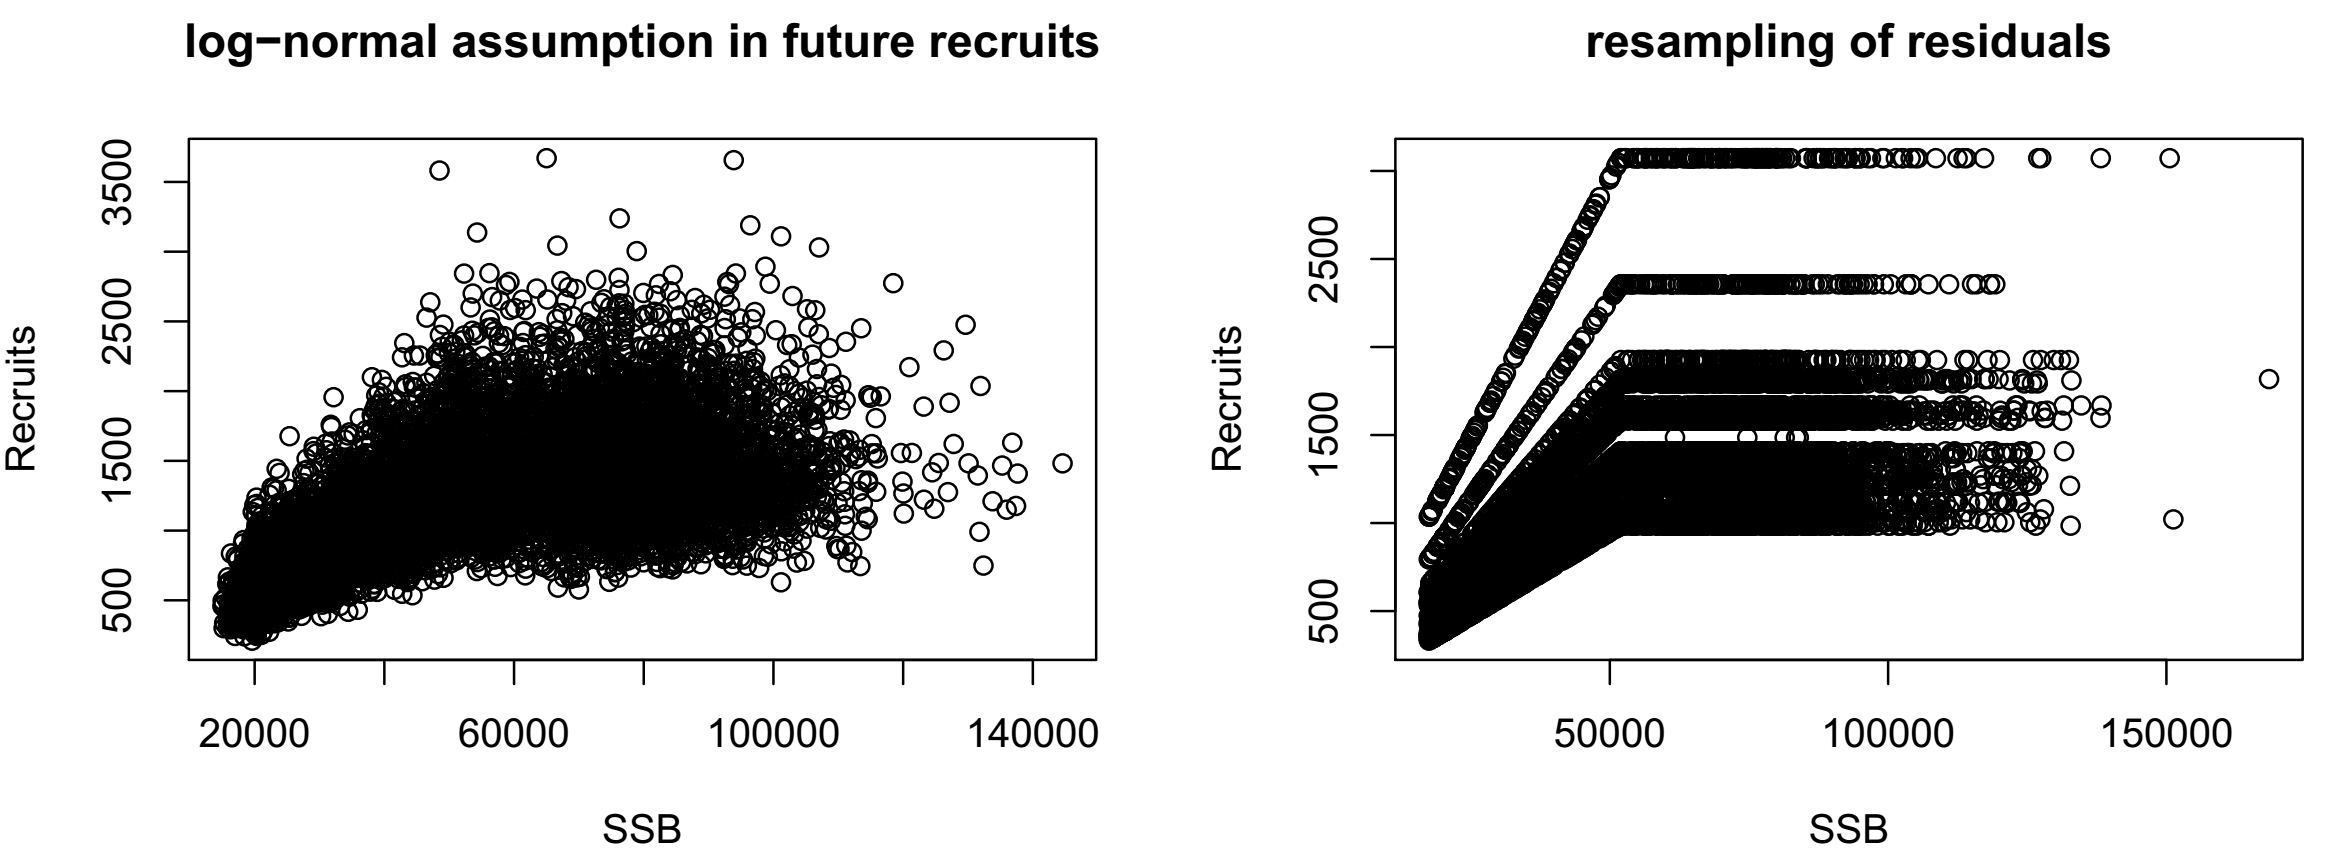
\includegraphics[bb=0 0 600 300, width=13cm]{fig_resample.png}
  \caption{将来予測における誤差分布の仮定の違い.(左) 対数正規分布の誤差を仮定した場合.(右) 残差のリサンプリングによる誤差を仮定した場合}
  \label{fig_resample}
\end{figure}

\begin{figure}[h]
  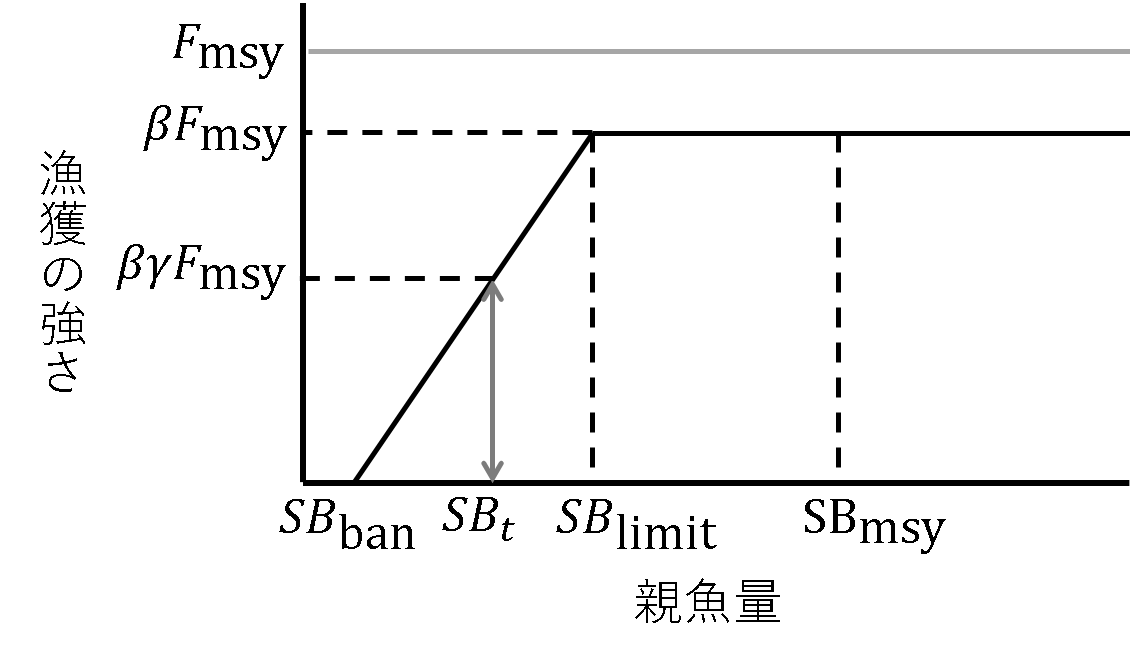
\includegraphics[bb=0 0 600 300, width=13cm]{fig_HCR.png}
  \caption{1系資源の漁獲制御ルールの模式図}
  \label{fig_HCR}
\end{figure}

\end{document}


\subsection{加入尾数の計算}
将来予測シミュレーションにおける$t$年($t>T_3$)の加入尾数$N_{t,S_{\mathrm{min}}}^k$ は
\begin{eqnarray}
  \log (N_{t,S_{\mathrm{min}}}^k ) = \log (\hat{N}_{t,S_{\mathrm{min}}}^k)+\rho [ \log (N_{t-1,S_{\mathrm{min}}}^k) - \log(\hat{N}_{t-1,S_{\mathrm{min}}^k}) ] + \varepsilon_t^k
\end{eqnarray}
で与えられる.ここで$\hat{N}_{t,S_{\mathrm{min}}}^k$は再生産関係式から得られる加入尾数の予測値,$\varepsilon_t^k$は$t$年における加入誤差である.$\varepsilon_t^k$は正規分布などの確率分布を仮定したり(式\ref{norm_recruit}),観測された残差をリサンプリング(式\ref{resample_recruit})したりする(図\ref{fig_resample}).正規分布の誤差を仮定する場合には
\begin{eqnarray}
  \varepsilon_t^k \sim \mathrm{Normal} (-0.5\sigma^2,(1-\rho^2 ) \sigma^2 )
  \label{norm_recruit}
\end{eqnarray}
となる\cite{johnson}.$\sigma^2$は,加入量と再生産関係の残差から以下の式で得られるものを使用する:
\begin{eqnarray}
  \sigma^2 = \frac{1}{T_2-T_{1}+1} \sum_{t=T_1}^{T_2} |\log (N_{t,S_{\mathrm{min}}}) -\log (\hat{N}_{t,S_{\mathrm{min}} } ) |
\end{eqnarray}
また,残差のリサンプリングを行う場合は
\begin{eqnarray}
  \varepsilon_t^k \sim (\mathrm{random} \quad \mathrm{draw} \quad \mathrm{from} \quad \varepsilon_{t={T_1,…,T_2}}) \\
  N_{t,S_{\mathrm{min}}}^k = \hat{N}_{t,S_{\mathrm{min}}}^k \exp( \varepsilon_t^k-\mathrm{mean}(\varepsilon_{t={T_1,…,T_2}}))
  \label{resample_recruit}
\end{eqnarray}
とする.ここで,$\varepsilon_t$は資源評価年における再生産関係の対数残差.残差の分布の仮定によらず,決定論的予測と確率分布の平均値が一致するように,平均値と中央値の違いを補正(式\ref{norm_recruit}では$-0.5\sigma^2$, 式\ref{resample_recruit}では $-\mathrm{mean}(\varepsilon_{t={T_1,…,T_2}})$に相当)する必要がある.推定資源量の不確実性が評価されている場合は,将来予測でもこれらの不確実性を考慮することが望ましい\cite{ichinokawa}.

